Our experiments use the squared exponential (SE) kernel, which has product
structure and can be used with D-SKIP; and the spline kernel, to which D-SKIP
does not directly apply. We use these kernels in tandem with D-SKI and D-SKIP
to achieve the fast MVMs derived in \cref{sgpdsec:met}.We write D-SE to denote the exact SE kernel with derivatives.

\subsection{Approximation Benchmark}
D-SKI and D-SKIP with the SE kernel approximate the original kernel well, both
in terms of MVM accuracy and spectral profile. Comparing D-SKI and D-SKIP to
their exact counterparts in Figure \ref{fig:error_ski}, we see their matrix
entries are very close (leading to MVM accuracy near $10^{-5}$), and their
spectral profiles are indistinguishable. The same is true with the spline
kernel.

\begin{figure}[ht]
  \begin{center}
    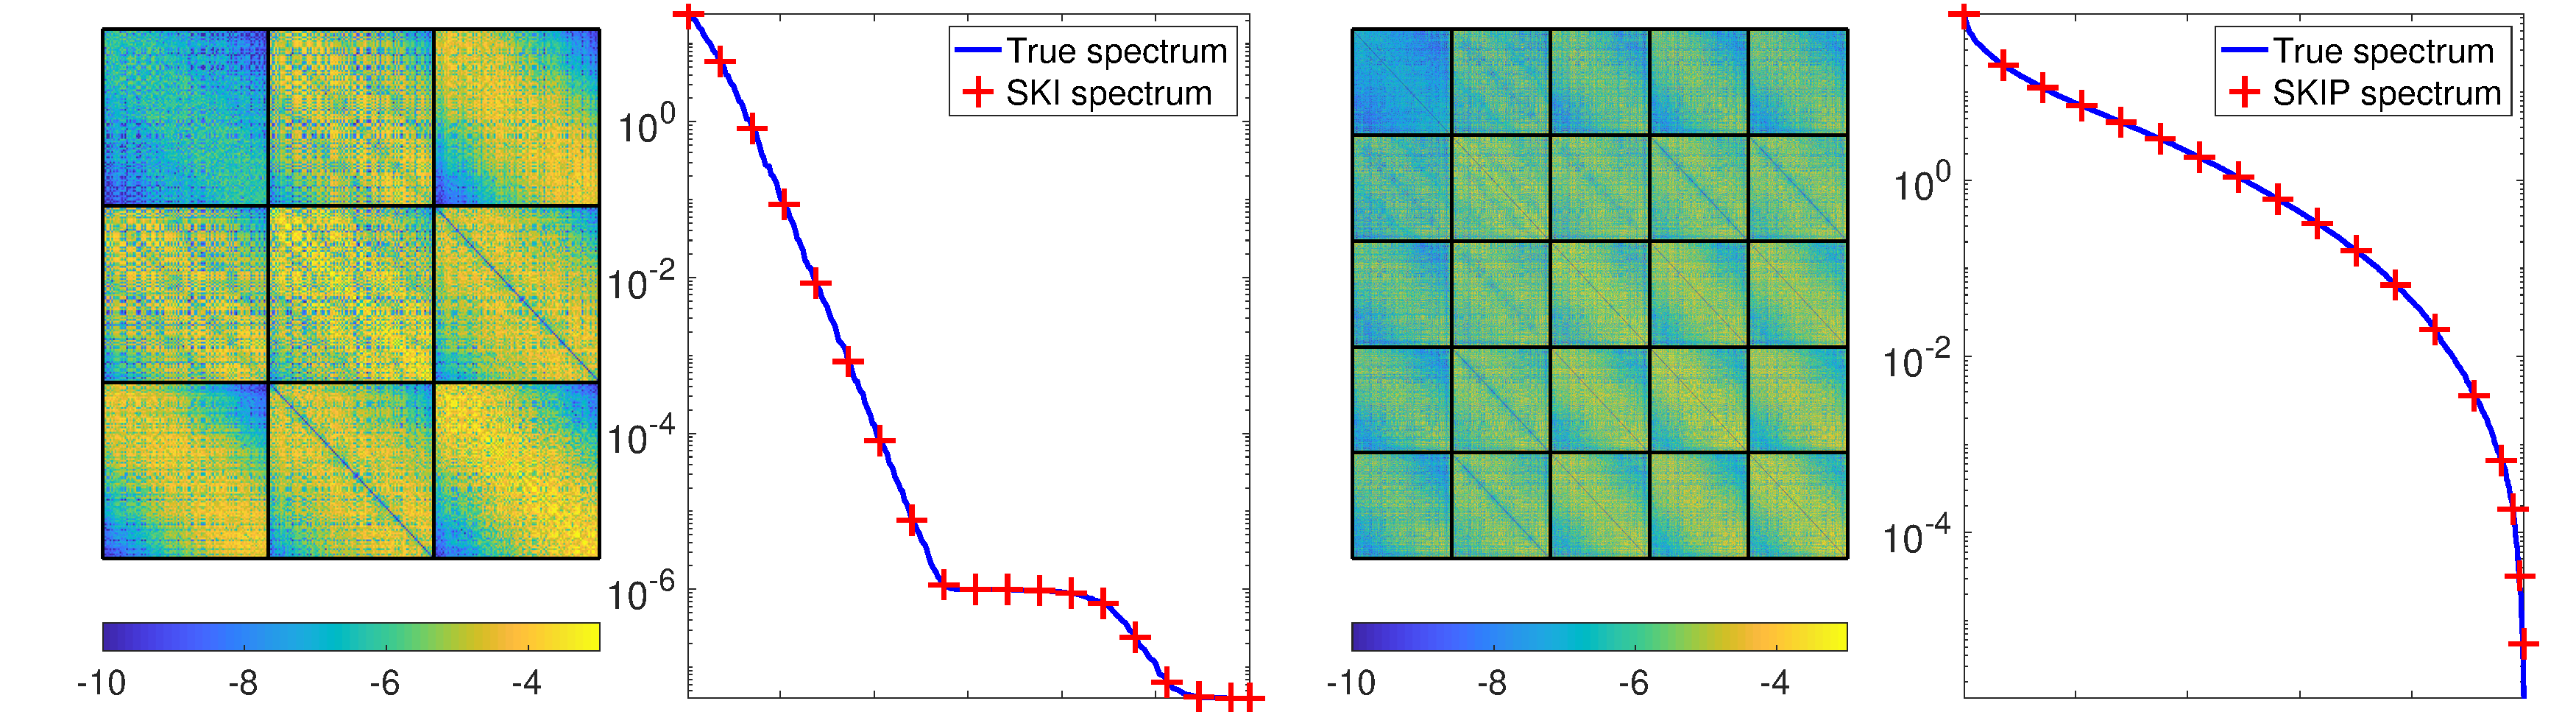
\includegraphics[width=0.98\textwidth]{./sgpd/pics/ski_error}
    \caption{(Left two images) $\log_{10}$ error in SKI approximation and
    comparison to the exact spectrum.(Right two images) $\log_{10}$ error in
    SKIP approximation and comparison to theexact spectrum.}
    \label{fig:error_ski}
  \end{center}
\end{figure}

Additionally, scaling tests in \cref{fig:scalingmvm} verify the predicted
complexity of D-SKI and D-SKIP. We show the relative fitting accuracy of SE,
SKI, D-SE, and D-SKI on some standard test functions in \cref{fig:testfncSKI}.


\begin{figure}[ht]
  \begin{center}
    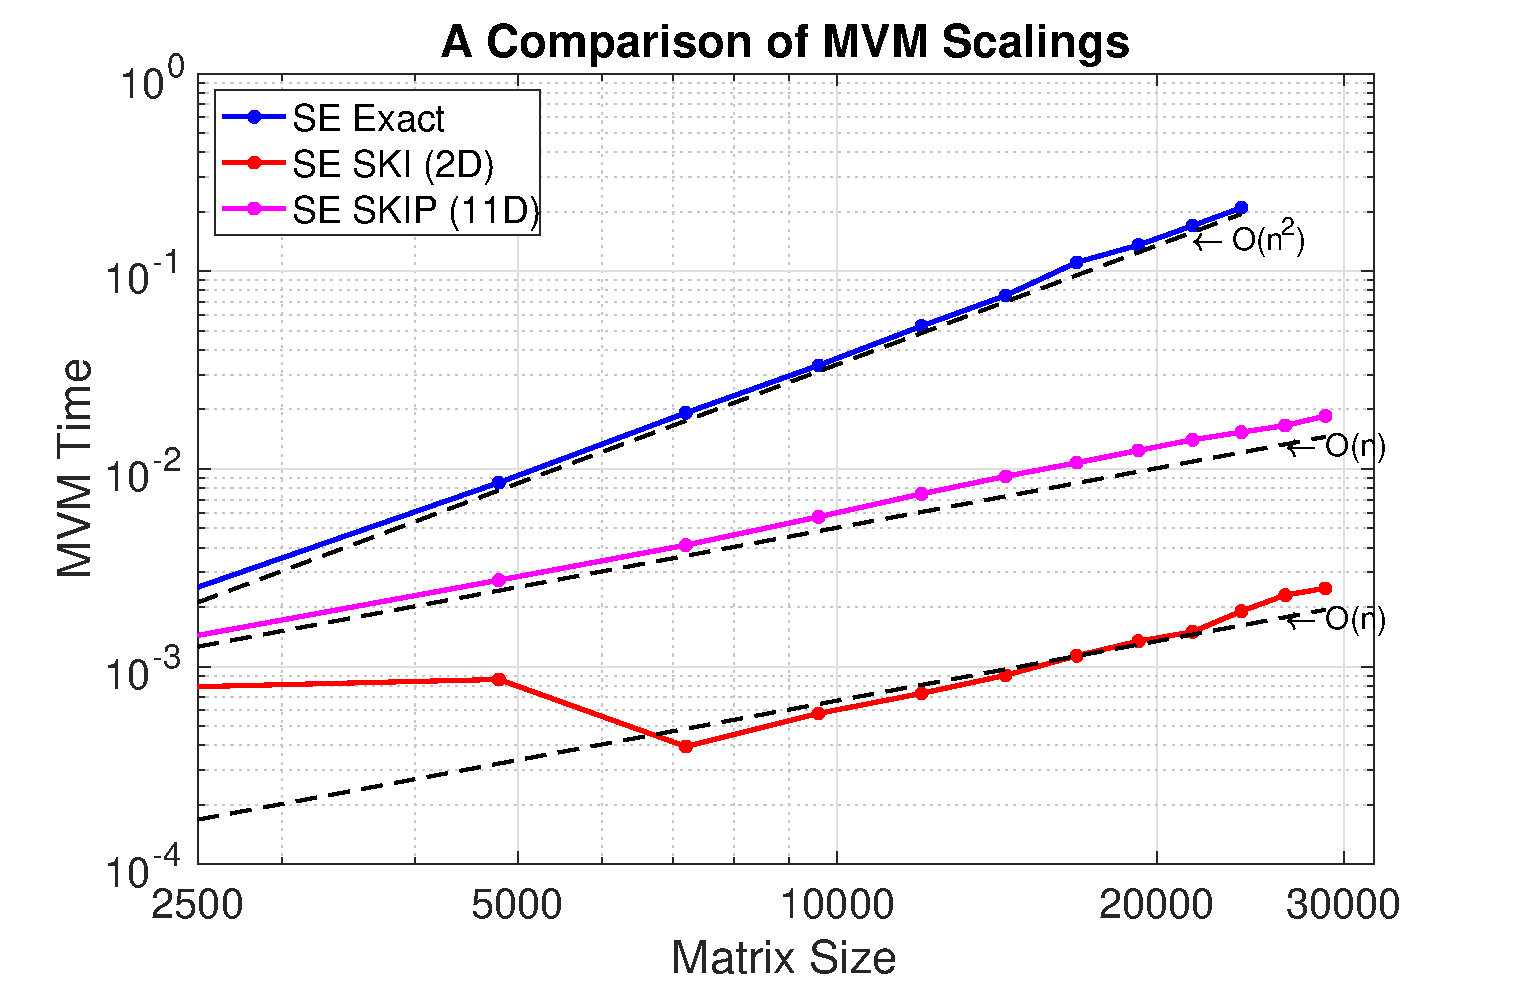
\includegraphics[width=\textwidth]{./sgpd/pics/mvmScaling}
    \caption{Scaling tests for D-SKI in two dimensions and D-SKIP in 11
    dimensions.D-SKIP uses fewer data points for identical matrix sizes.}
    \label{fig:scalingmvm}
  \end{center}
\end{figure}

\begin{table}[ht]
  \centering
  \caption{Relative RMSE on Test Functions Using SKI and
  Derivatives\textsuperscript{$\alpha$}.}\label{fig:testfncSKI}
  \begin{threeparttable}
    \begin{tabular}{r c c c c c c}
      \toprule 
      & Branin & Franke & Sine Norm & Sixhump & StyTang & Hart3 \\ \midrule
      SE & 6.02e-3 & 8.73e-3 & 8.64e-3 & 6.44e-3 & 4.49e-3 & 1.30e-2 \\
      SKI & 3.97e-3 & 5.51e-3 & 5.37e-3 & 5.11e-3 & 2.25e-3 & 8.59e-3 \\
      D-SE & 1.83e-3 & 1.59e-3 & 3.33e-3 & 1.05e-3 & 1.00e-3 & 3.17e-3 \\
      D-SKI & 1.03e-3 & 4.06e-4 & 1.32e-3 & 5.66e-4 & 5.22e-4 & 1.67e-3 \\ 
      \bottomrule
    \end{tabular}
    \begin{tablenotes}
      \item[$\alpha$]Relative RMSE error measured on 10000 testing points. Test
      functions from~\cite{sfutest2013} includes five 2D functions (Branin,
      Franke, Sine Norm, Sixhump, and Styblinski-Tang) and one 3D function 
      (Hartman). We train the SE kernel on $4000$ points, the D-SE kernel on
      $4000/(d+1)$ points, and SKI and D-SKI with SE kernel on $10000$ points to
      achieve comparable runtimes between methods.
    \end{tablenotes}
  \end{threeparttable}
\end{table}

\subsection{Dimensionality reduction}

We apply active subspace pre-processing to the 20 dimensional Welsh test
function in \cite{ben2007modeling}. The top six eigenvalues of its gradient
covariance matrix are well separated from the rest as seen in 
\cref{fig:dir_var}. However, the function is far from smooth  when projected
onto the leading 1D or 2D active subspace, as \crefrange{fig:d1_sca}
{fig:joint_sca} indicates, where the color shows the function value.
\begin{figure}[ht]
  \begin{center}
    \begin{subfigure}{0.47\textwidth}
      \centering
      \captionsetup{justification=centering}
      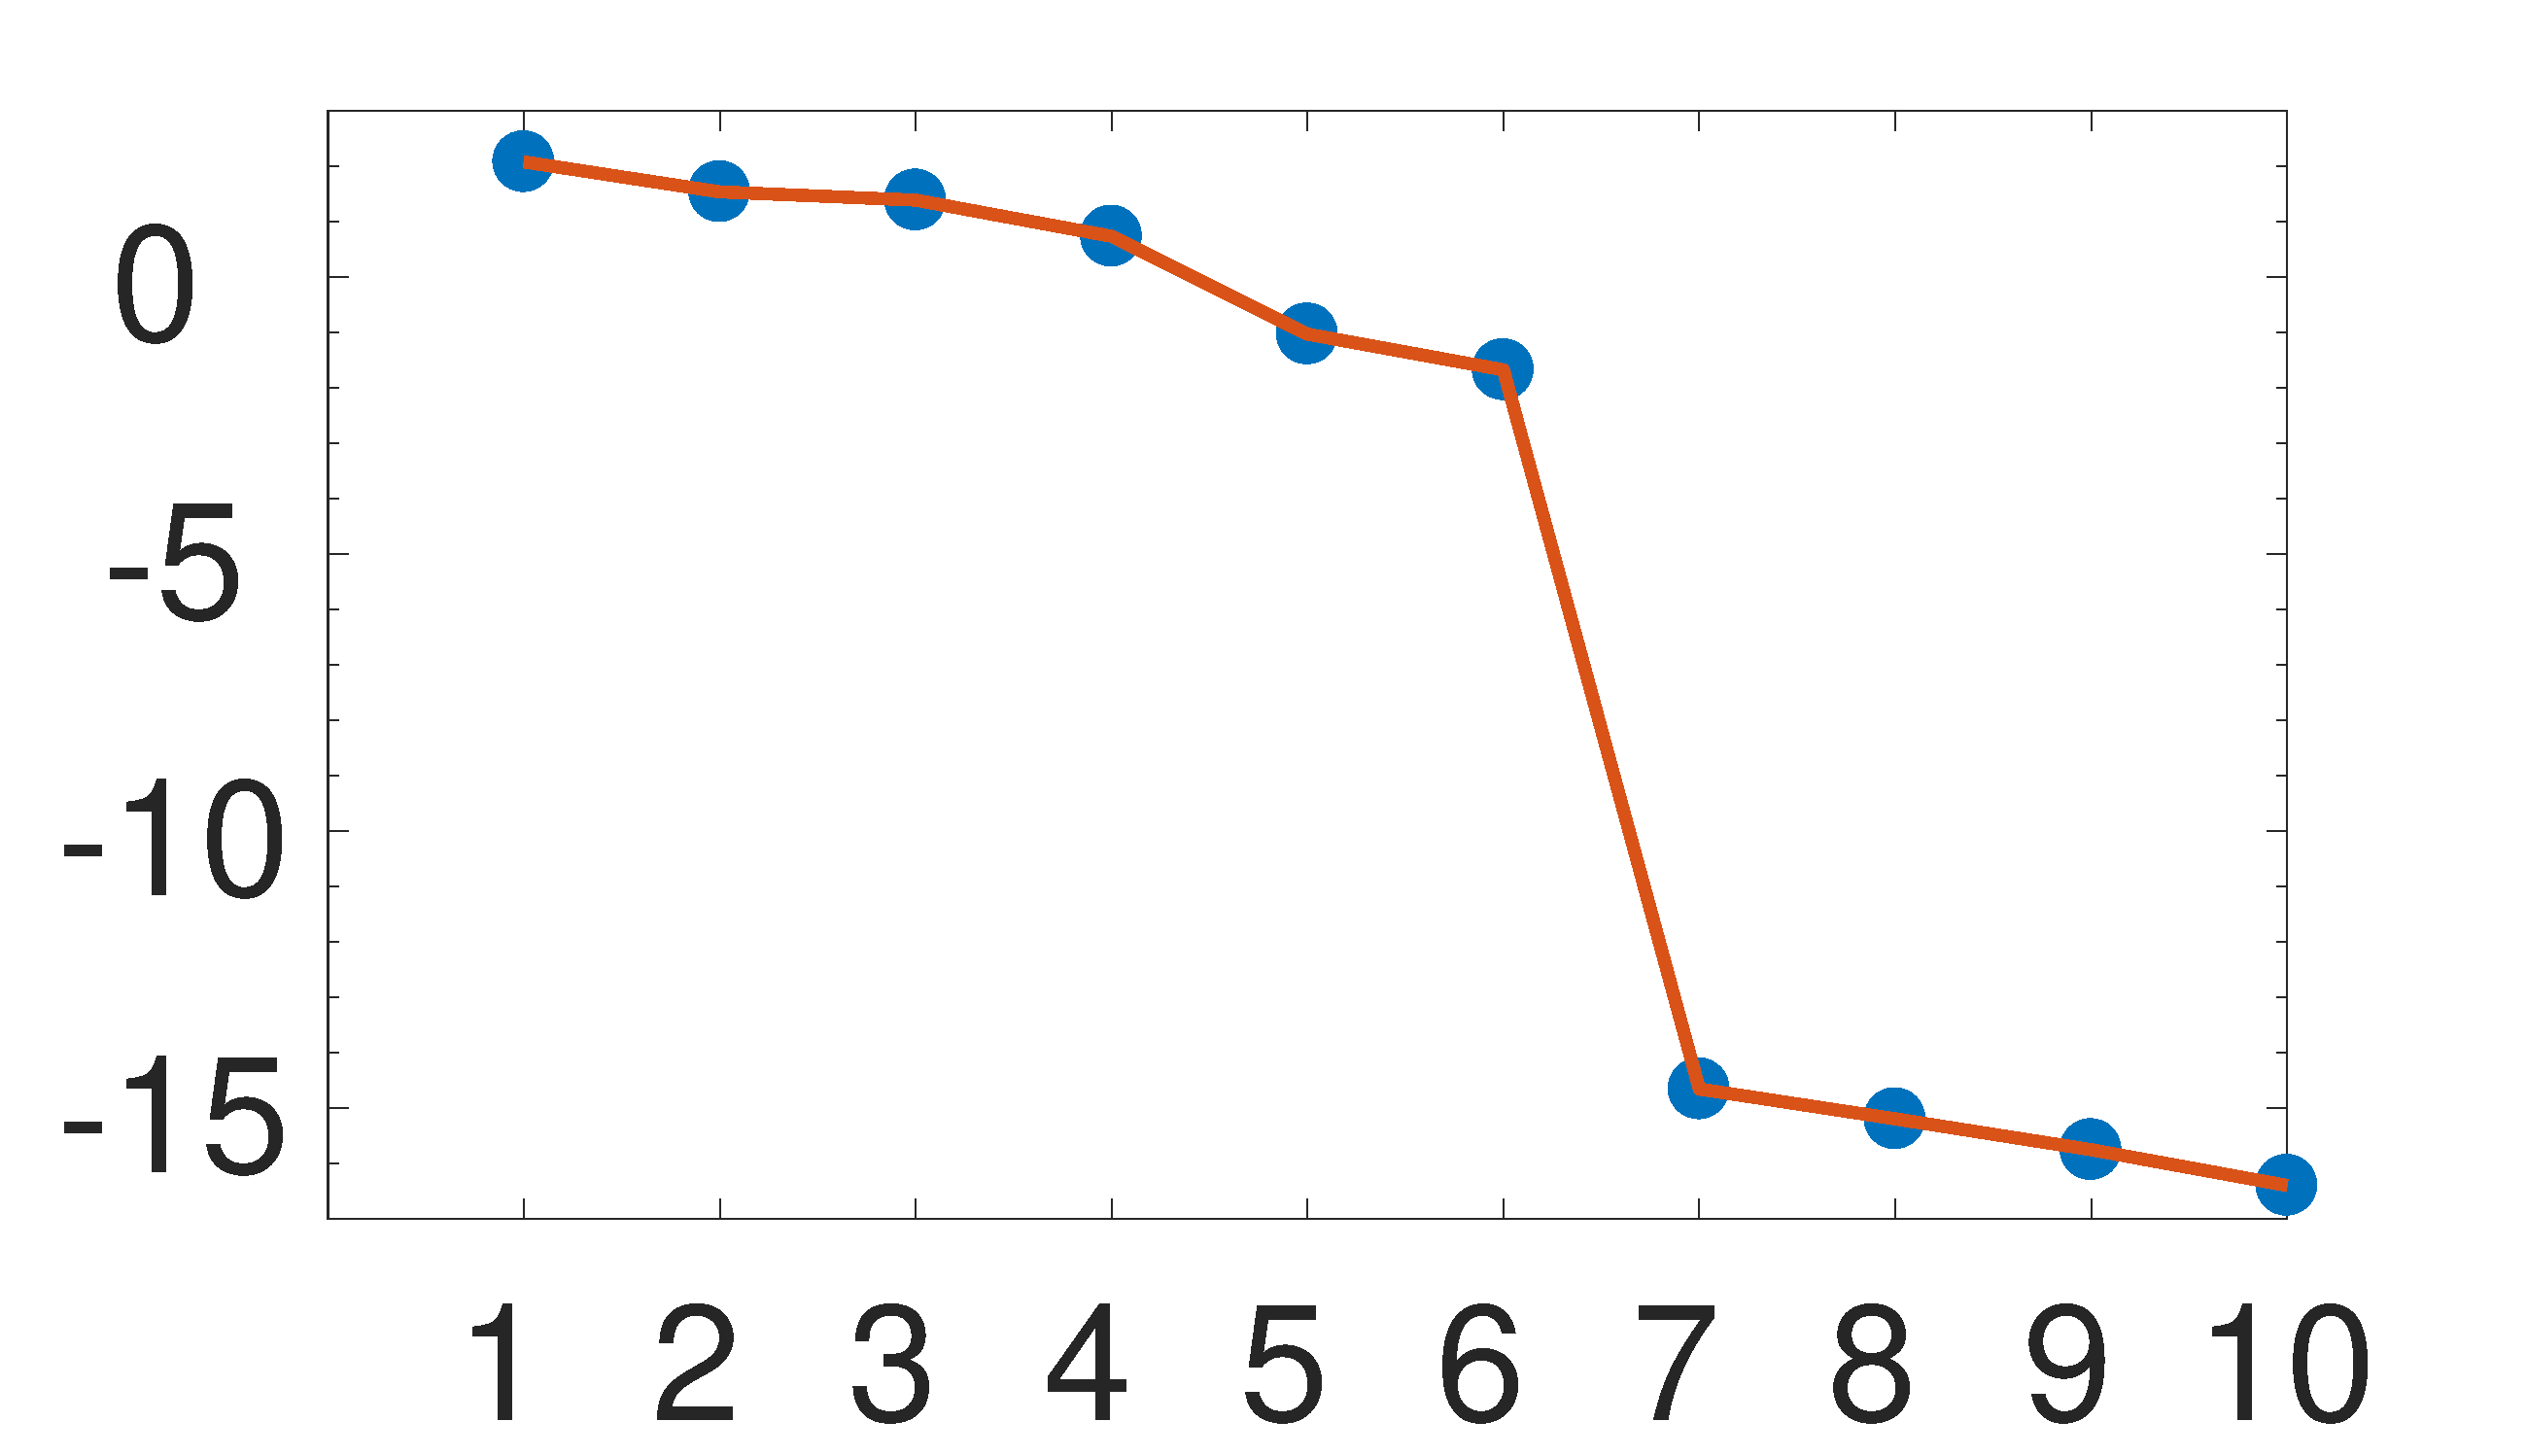
\includegraphics[width=\textwidth,trim=1cm .5cm 2.5cm 1.5cm,clip]
      {./sgpd/pics/dir_var}
      \caption{Log Directional Variation}\label{fig:dir_var}
    \end{subfigure}
    %
    \begin{subfigure}{0.47\textwidth}
      \centering
      \captionsetup{justification=centering}
      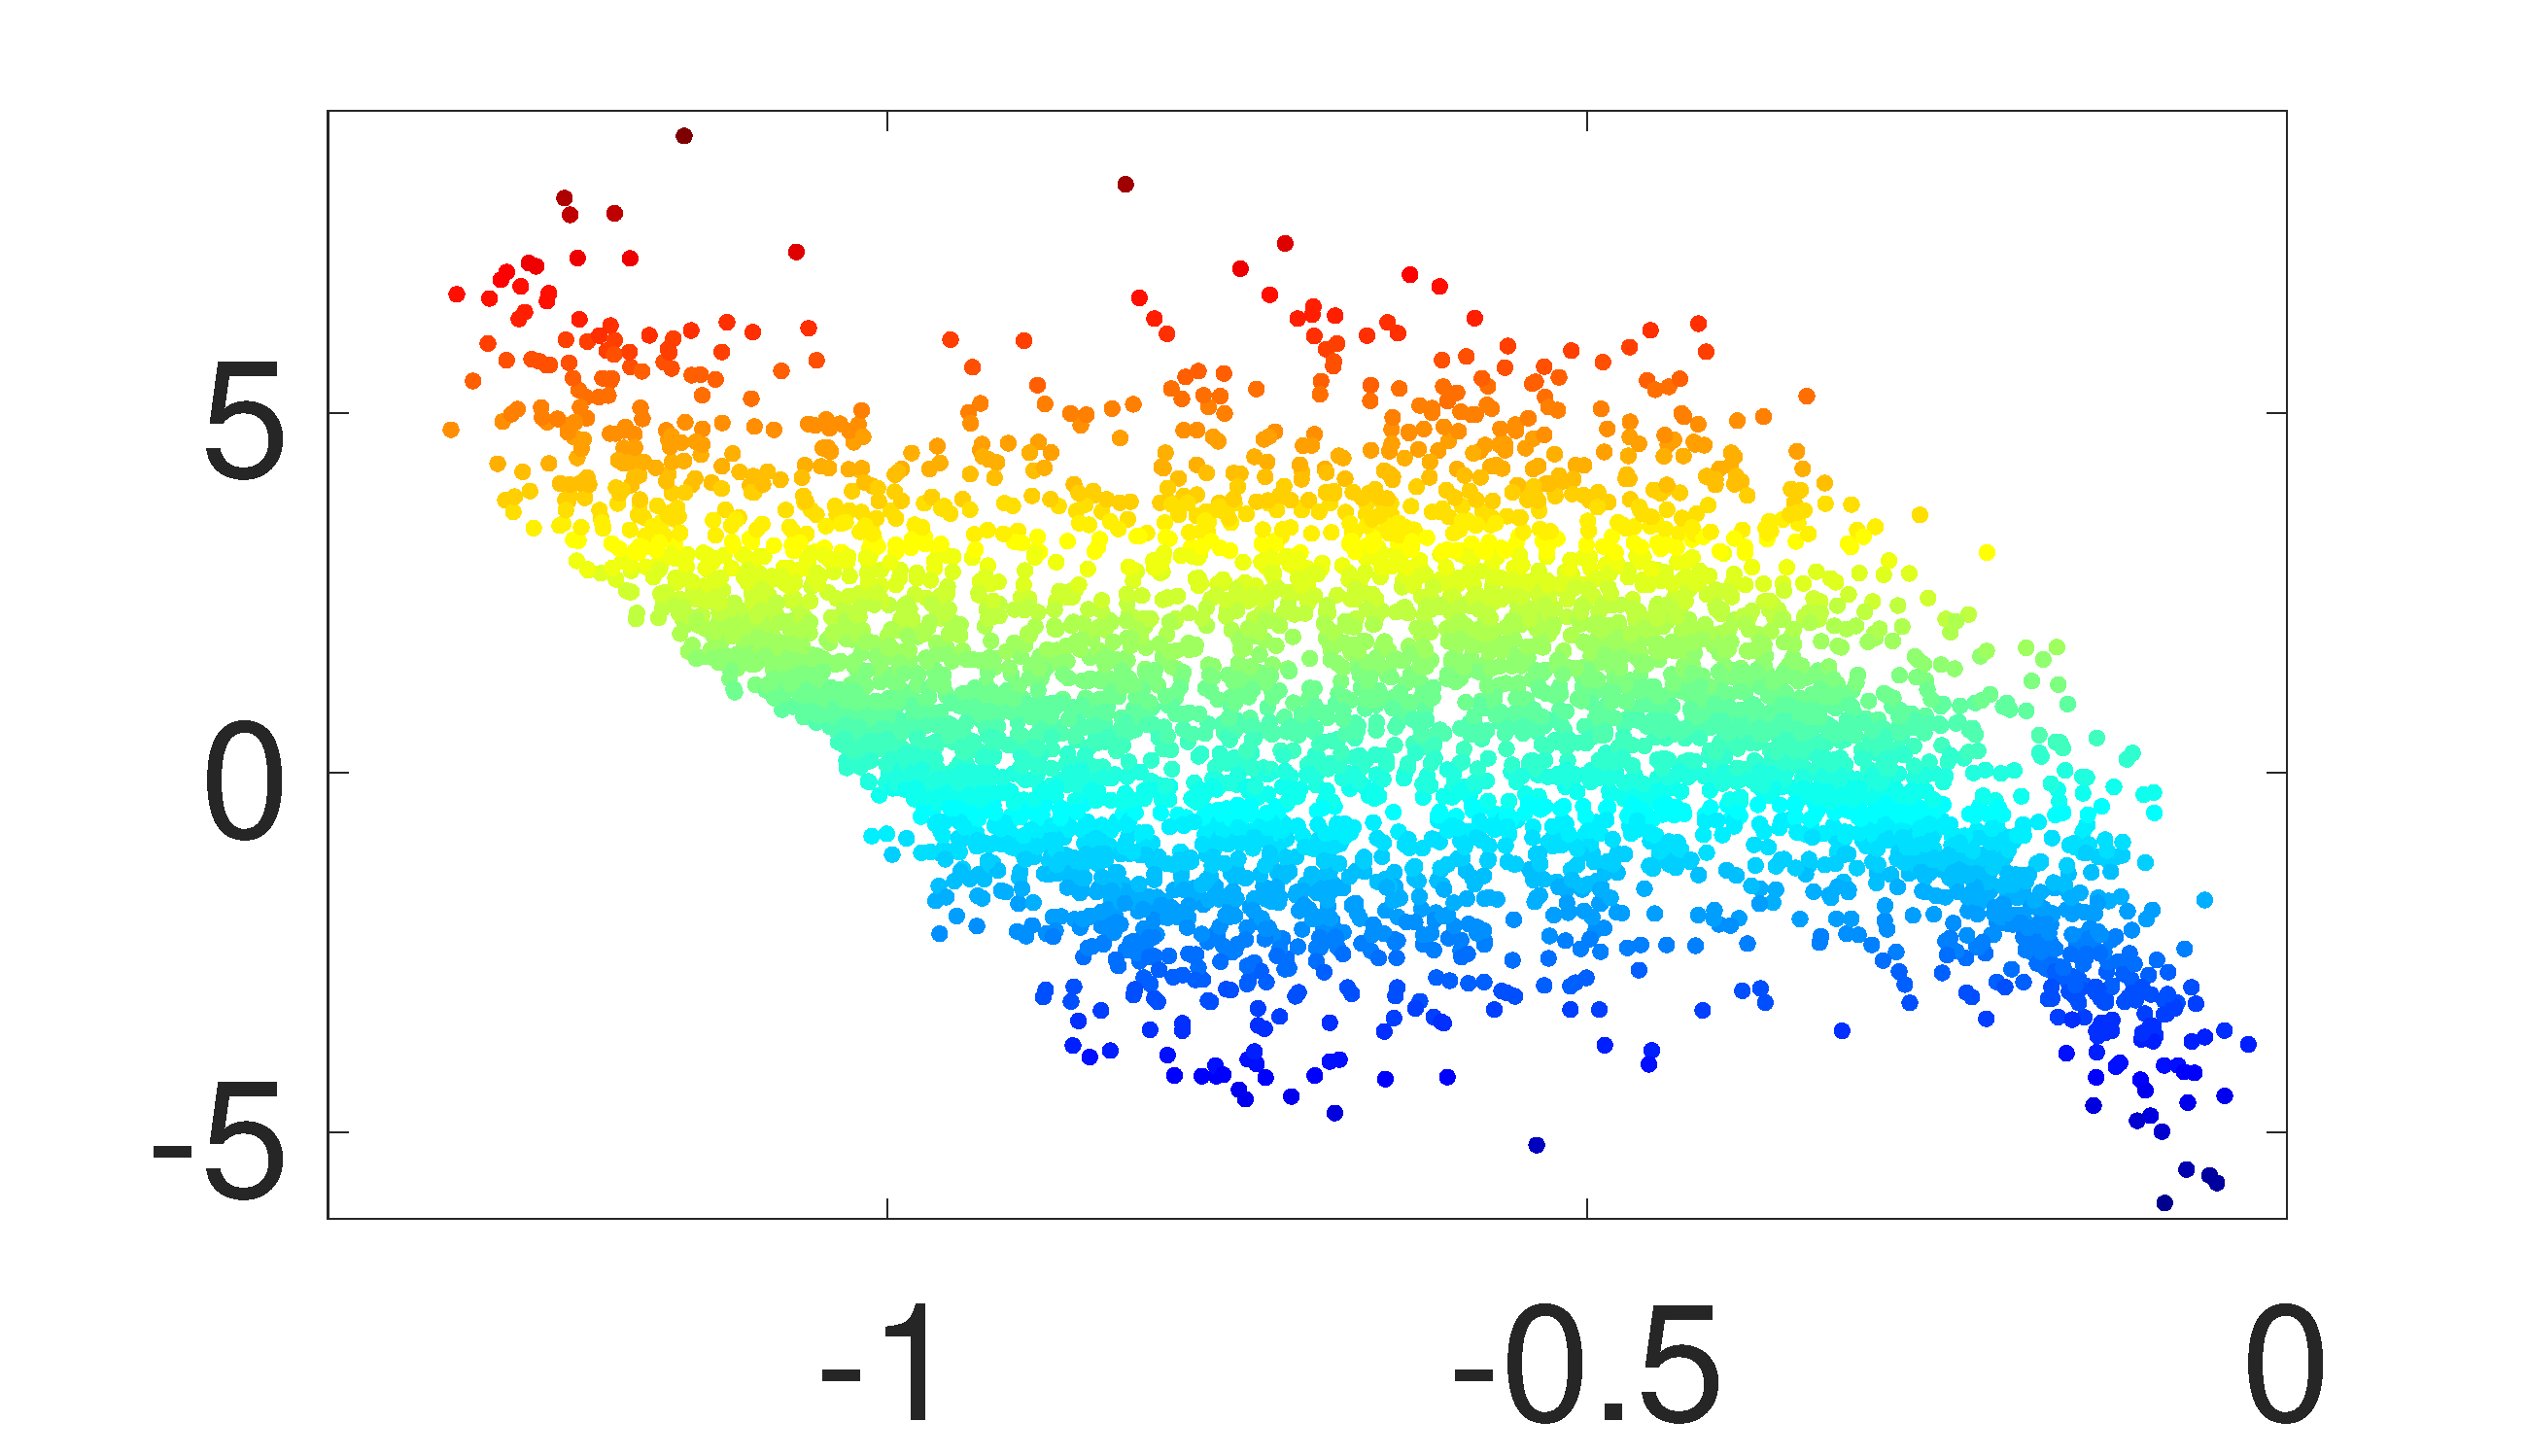
\includegraphics[width=\textwidth,trim=1cm .5cm 2.5cm 1.5cm,clip]
      {./sgpd/pics/d1scatter}
      \caption{First Active Direction}\label{fig:d1_sca}
    \end{subfigure}
    %
    \begin{subfigure}{0.47\textwidth}
      \centering
      \captionsetup{justification=centering}
      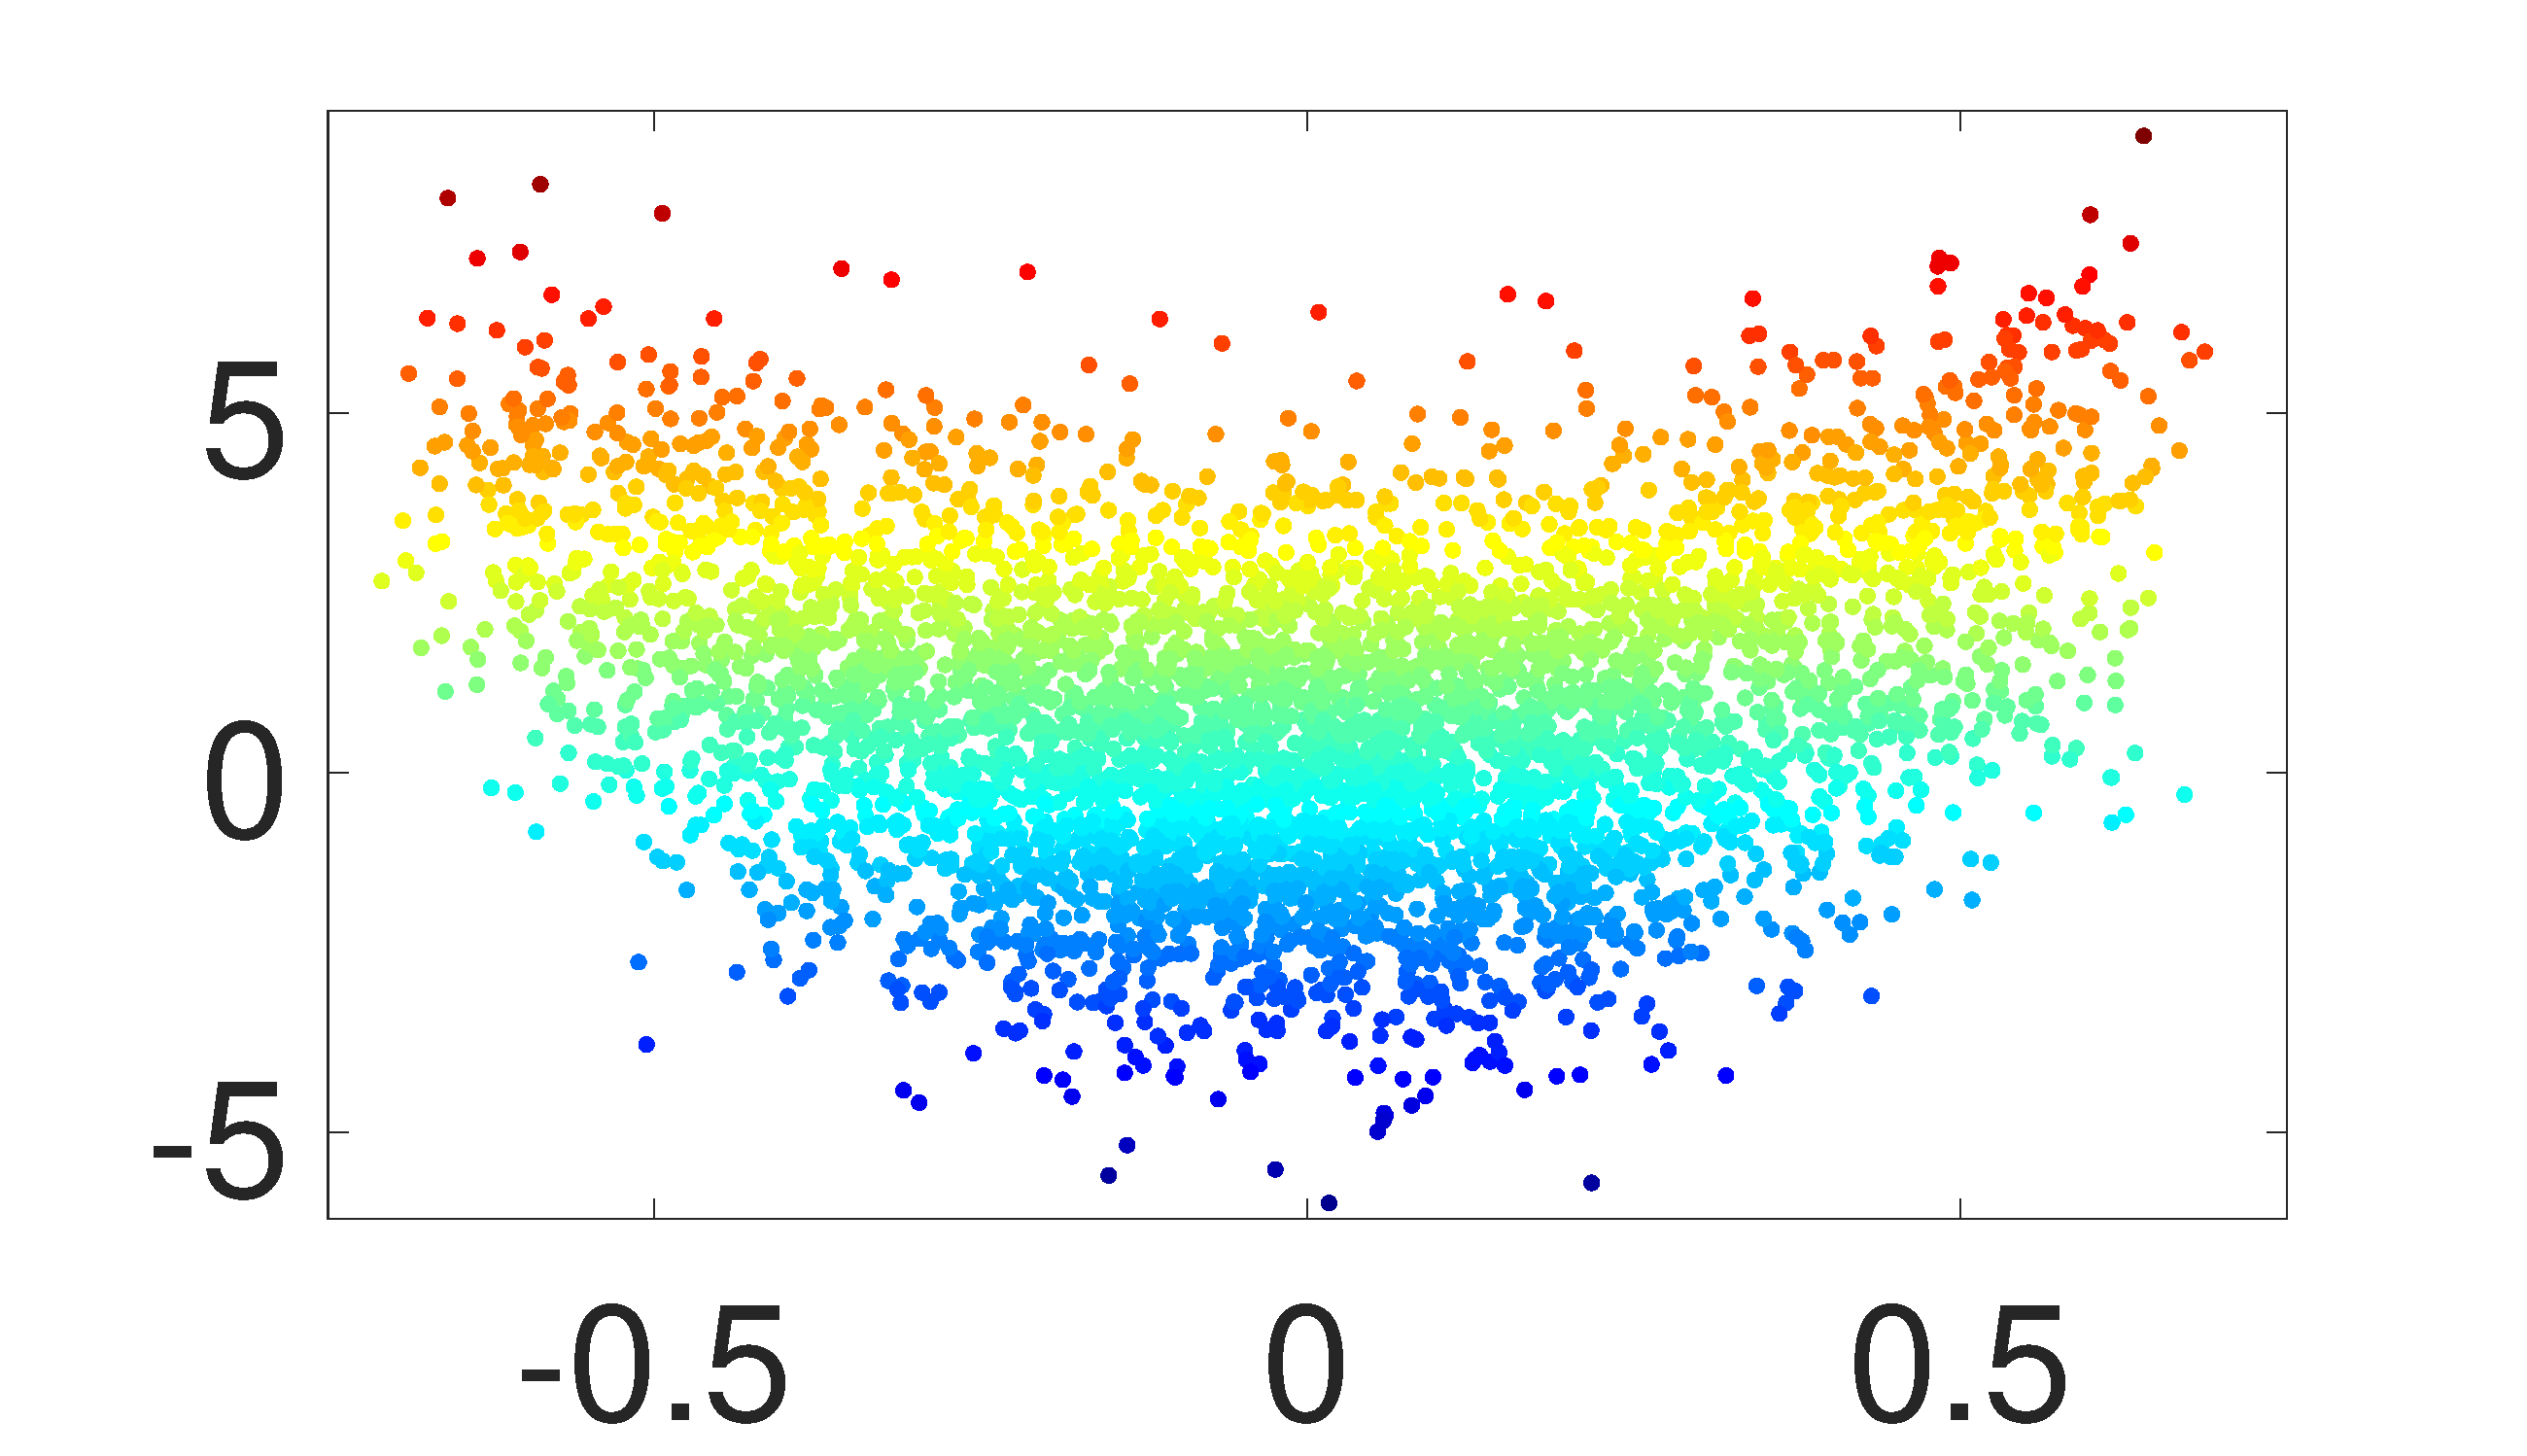
\includegraphics[width=\textwidth,trim=1cm .5cm 2.5cm 1.5cm,clip]
      {./sgpd/pics/d2scatter}
      \caption{Second Active Direction}\label{fig:d2_sca}
    \end{subfigure}
    %
    \begin{subfigure}{0.47\textwidth}
      \centering
      \captionsetup{justification=centering}
      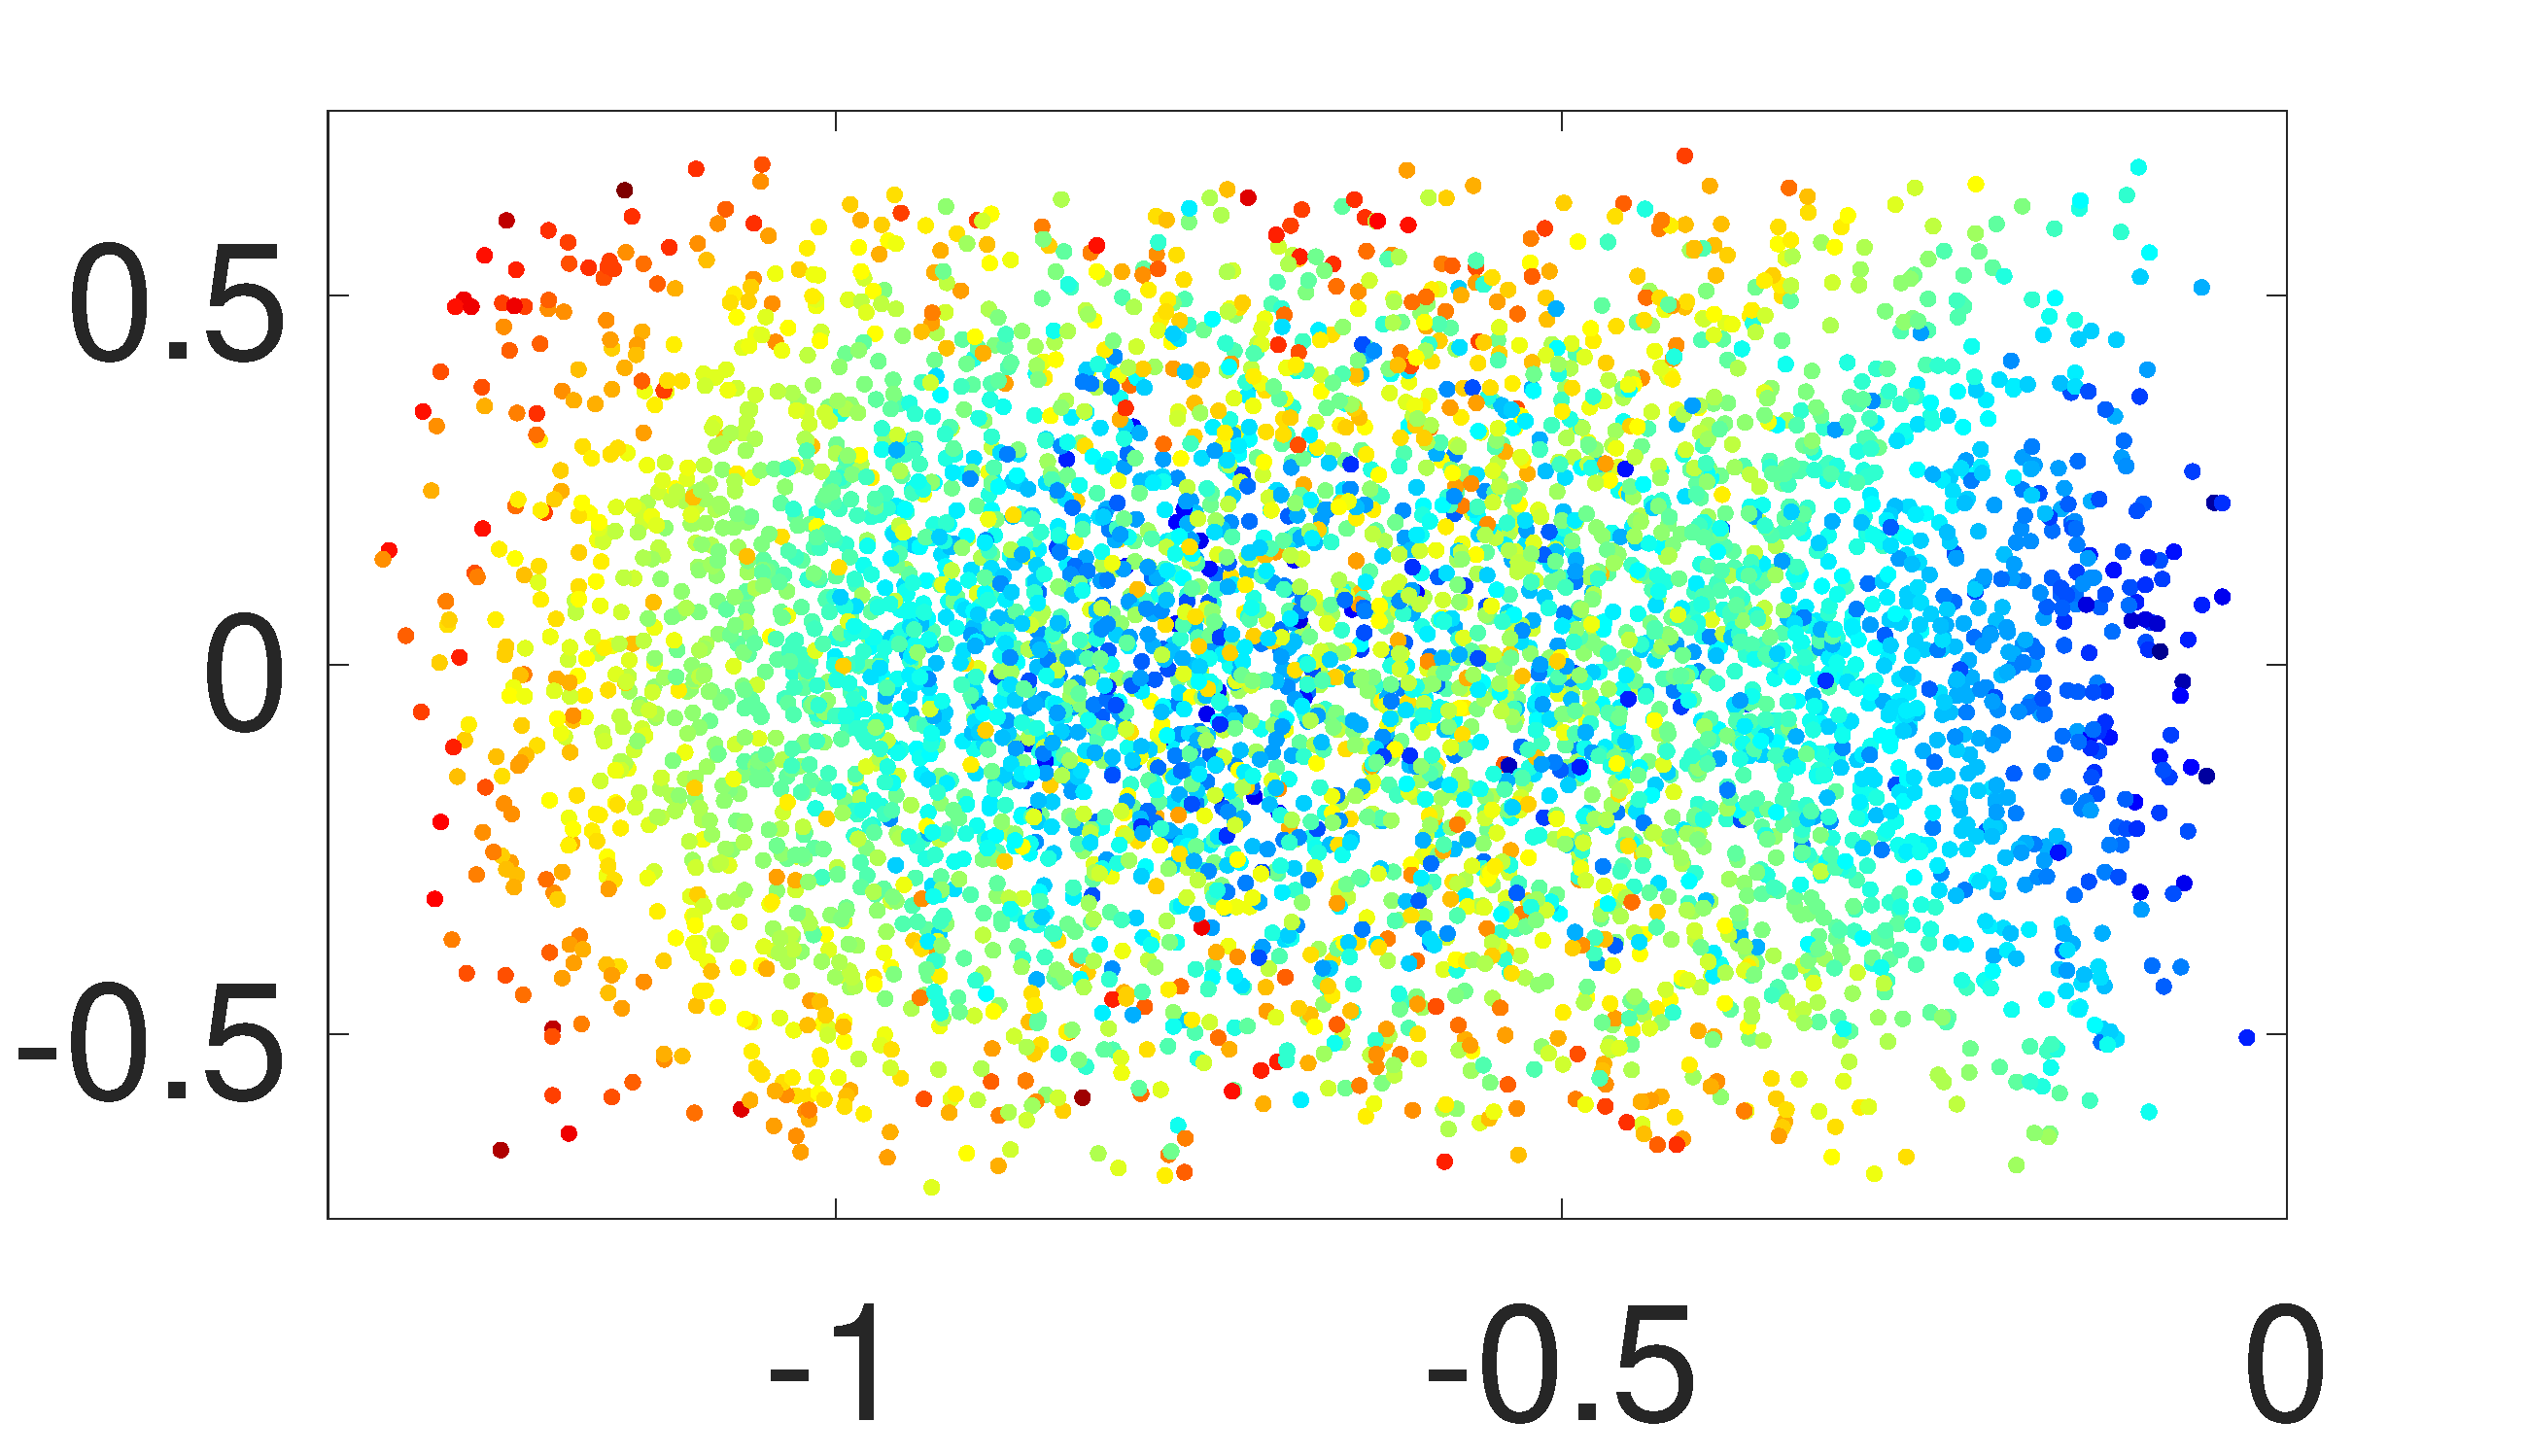
\includegraphics[width=\textwidth,trim=1cm .5cm 2.5cm 1.5cm,clip]
      {./sgpd/pics/jointscatter}
      \caption{Leading 2D Active Subspace}\label{fig:joint_sca}
    \end{subfigure}
    \caption{\cref{fig:dir_var} shows the top $10$ eigenvalues of the gradient
    covariance. Welsh is projected onto the first and second active direction in
    \ref{fig:d1_sca} and \ref{fig:d2_sca}. After joining them together, we see
    in \ref{fig:joint_sca} that points of different color are highly mixed, indicating a very spiky surface.} \label{fig:dim_red}
  \end{center}
\end{figure}

We therefore apply D-SKI and D-SKIP on the 3D and 6D active subspace,
respectively, using $5000$ training points, and compare the prediction error
against D-SE with $190$ training points because of our scaling advantage. 
\cref{tab:dim_red} reveals that while the 3D active subspace fails to capture
all the variation of the function, the 6D active subspace is able to do so.
These properties are demonstrated by the poor prediction of D-SKI in 3D and the
excellent prediction of D-SKIP in 6D. 

\begin{table}[ht]
  \centering
  \caption{Relative RMSE and SMAE prediction error for Welsh
  \textsuperscript{$\alpha$}.}\label{tab:dim_red}
  \begin{threeparttable}
    \begin{tabular}{r c c c}
      \toprule
      & D-SE & D-SKI (3D) & D-SKIP (6D) \\ \midrule
      RMSE & 4.900e-02 & 2.267e-01 & 3.366e-03 \\
      SMAE & 4.624e-02 & 2.073e-01 & 2.590e-03 \\
      \bottomrule
    \end{tabular}
    \begin{tablenotes}
      \item[$\alpha$]The D-SE kernel is trained on $4000/(d+1)$ points, with
      D-SKI and D-SKIP trained on $5000$ points. The 6D active subspace is
      sufficient to capture the variation of the test function.
    \end{tablenotes}
  \end{threeparttable}
\end{table}



\subsection{Rough terrain reconstruction}

Rough terrain reconstruction is a key application in robotics 
\cite{gingras2010rough, konolige2010large}, autonomous navigation 
\cite{hadsell2010accurate}, and geostatistics. Through a set of terrain
measurements, the problem is to predict the underlying topography of some
region. In the following experiment, we consider roughly $23$ million
non\hyp{}uniformly sampled elevation measurements of Mount St. Helens obtained
via LiDAR \cite{sthelen2002lidar}. We bin the measurements into a $970\times
950$ grid, and downsample to a $120\Times 117$ grid. Derivatives are
approximated using a finite difference scheme.

\begin{figure}[ht]
  \begin{center}
    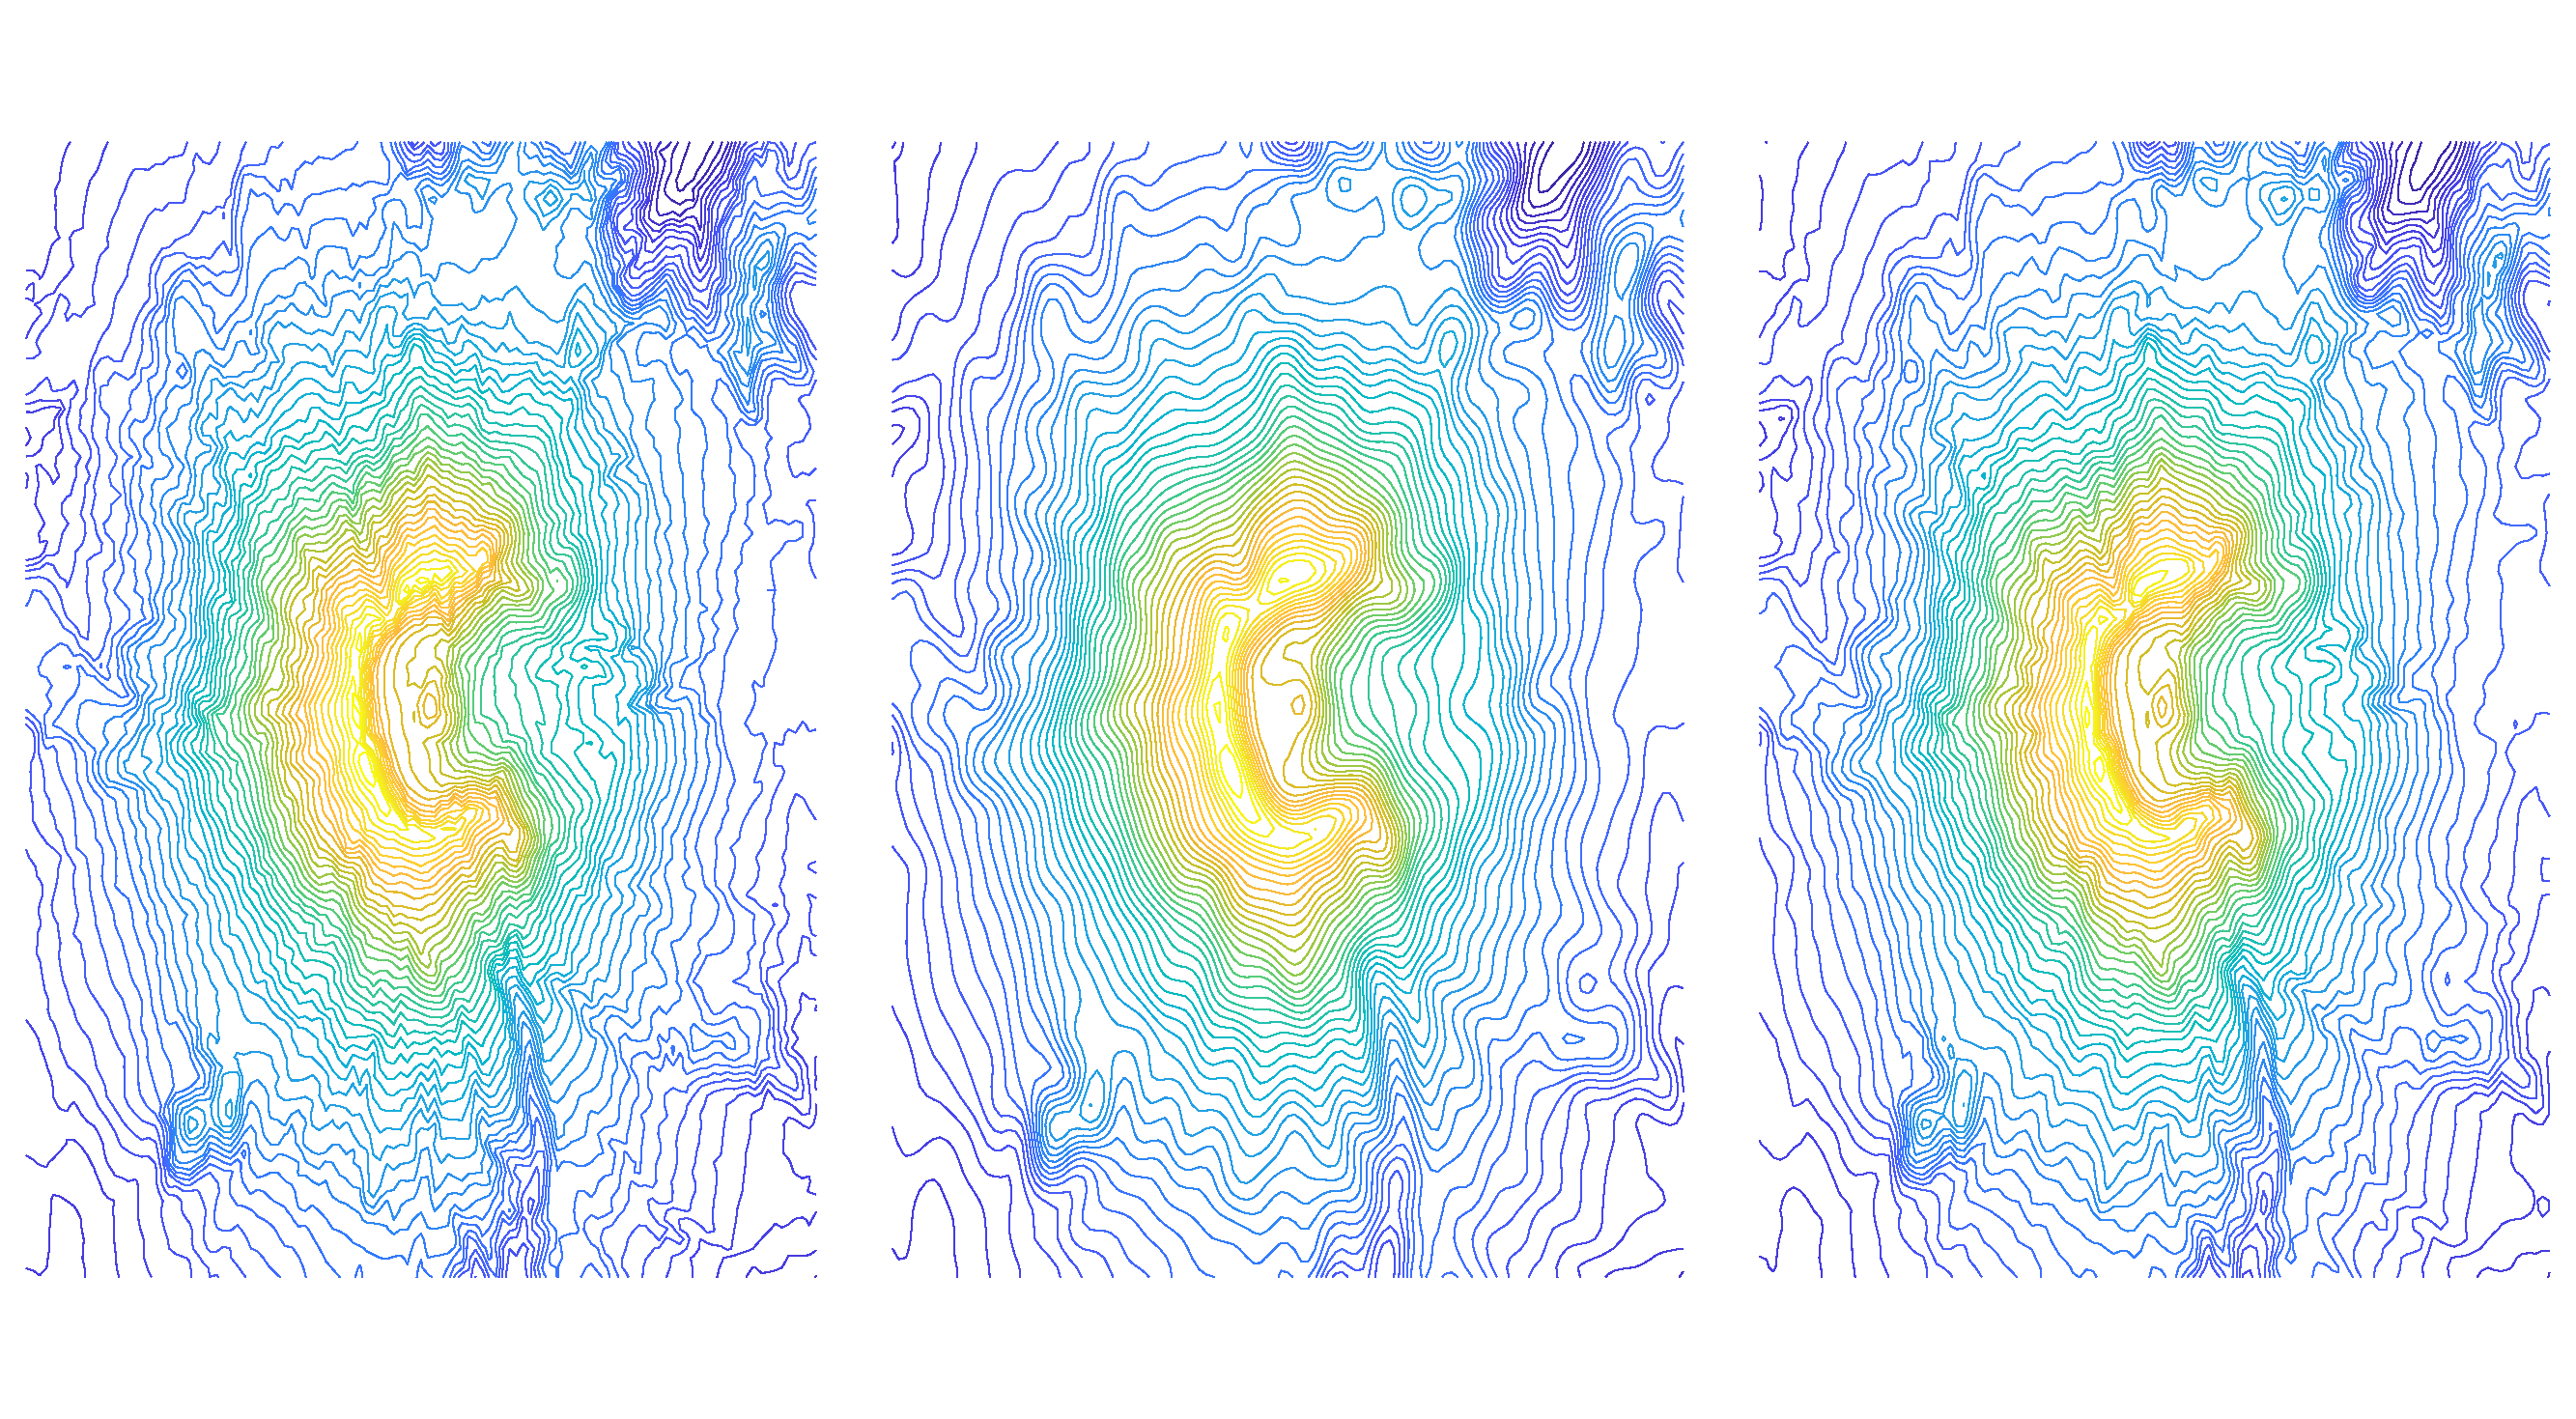
\includegraphics[width=\textwidth, height=0.47\textwidth, trim = 0cm 0cm 0cm
    0cm,clip]{./sgpd/pics/mountainContour}
    \caption{On the left is the true elevation map of Mount St. Helens. In the
    middle is the elevation map calculated with the SKI. On the right is the
    elevation map calculated with D-SKI.}\label{fig:MtSH_map}
  \end{center}
\end{figure}

We randomly select $90\%$ of the grid for training and the remainder for
testing. We do not include results for D-SE, as its kernel matrix has dimension
roughly $4\Times10^4$. We plot contour maps predicted by SKI and D-SKI
in \cref{fig:MtSH_map} --- the latter looks far closer to the ground truth
than the former. This is quanitified in the following table:

\begin{table}[ht]
  \centering
  \caption{Hyperparameters Recovered, Recovery SMAE, and Recovery Time for SKI
  and D-SKI on Mountain St. Helens Data\textsuperscript{$\alpha$}.}
  \label{tab:mtsthelens}
  \begin{threeparttable}
    \begin{tabular}{r c c c c c c c}
      \toprule
      & $\ell$ & $s$ & $\sigma_1$ & $\sigma_2$ & SMAE\textsubscript{test} &
      SMAE\textsubscript{all} & Time[s]\\ \midrule
      SKI & 35.196 & 207.689 & 12.865 & n.a. & 0.0308 & 0.0357 & 37.67\\
      D-SKI & 12.630 & 317.825 & 6.446 & 2.799 & 0.0165 & 0.0254 & 131.70\\
      \bottomrule
    \end{tabular}
    \begin{tablenotes}
      \item[$\alpha$] $\sigma_1$ and $\sigma_2$ are the noise parameters for
      value and gradient, respectively.
    \end{tablenotes}
  \end{threeparttable}
\end{table}

\subsection{Implicit surface reconstruction}
Reconstructing surfaces from point cloud data and surface normals is a standard
problem in computer vision and graphics. One popular approach is to fit an
implicit function that is zero on the surface with gradients equal to the
surface normal. Local Hermite RBF interpolation has been considered
in prior work \cite{macedo2011hermite}, but this approach is sensitive to noise.
In our experiments, using a GP instead of splining reproduces implicit surfaces
with very high accuracy.  In this case, a GP with derivative information is
required, as the function values are all zero.

\begin{figure}[ht]
  \begin{center}
    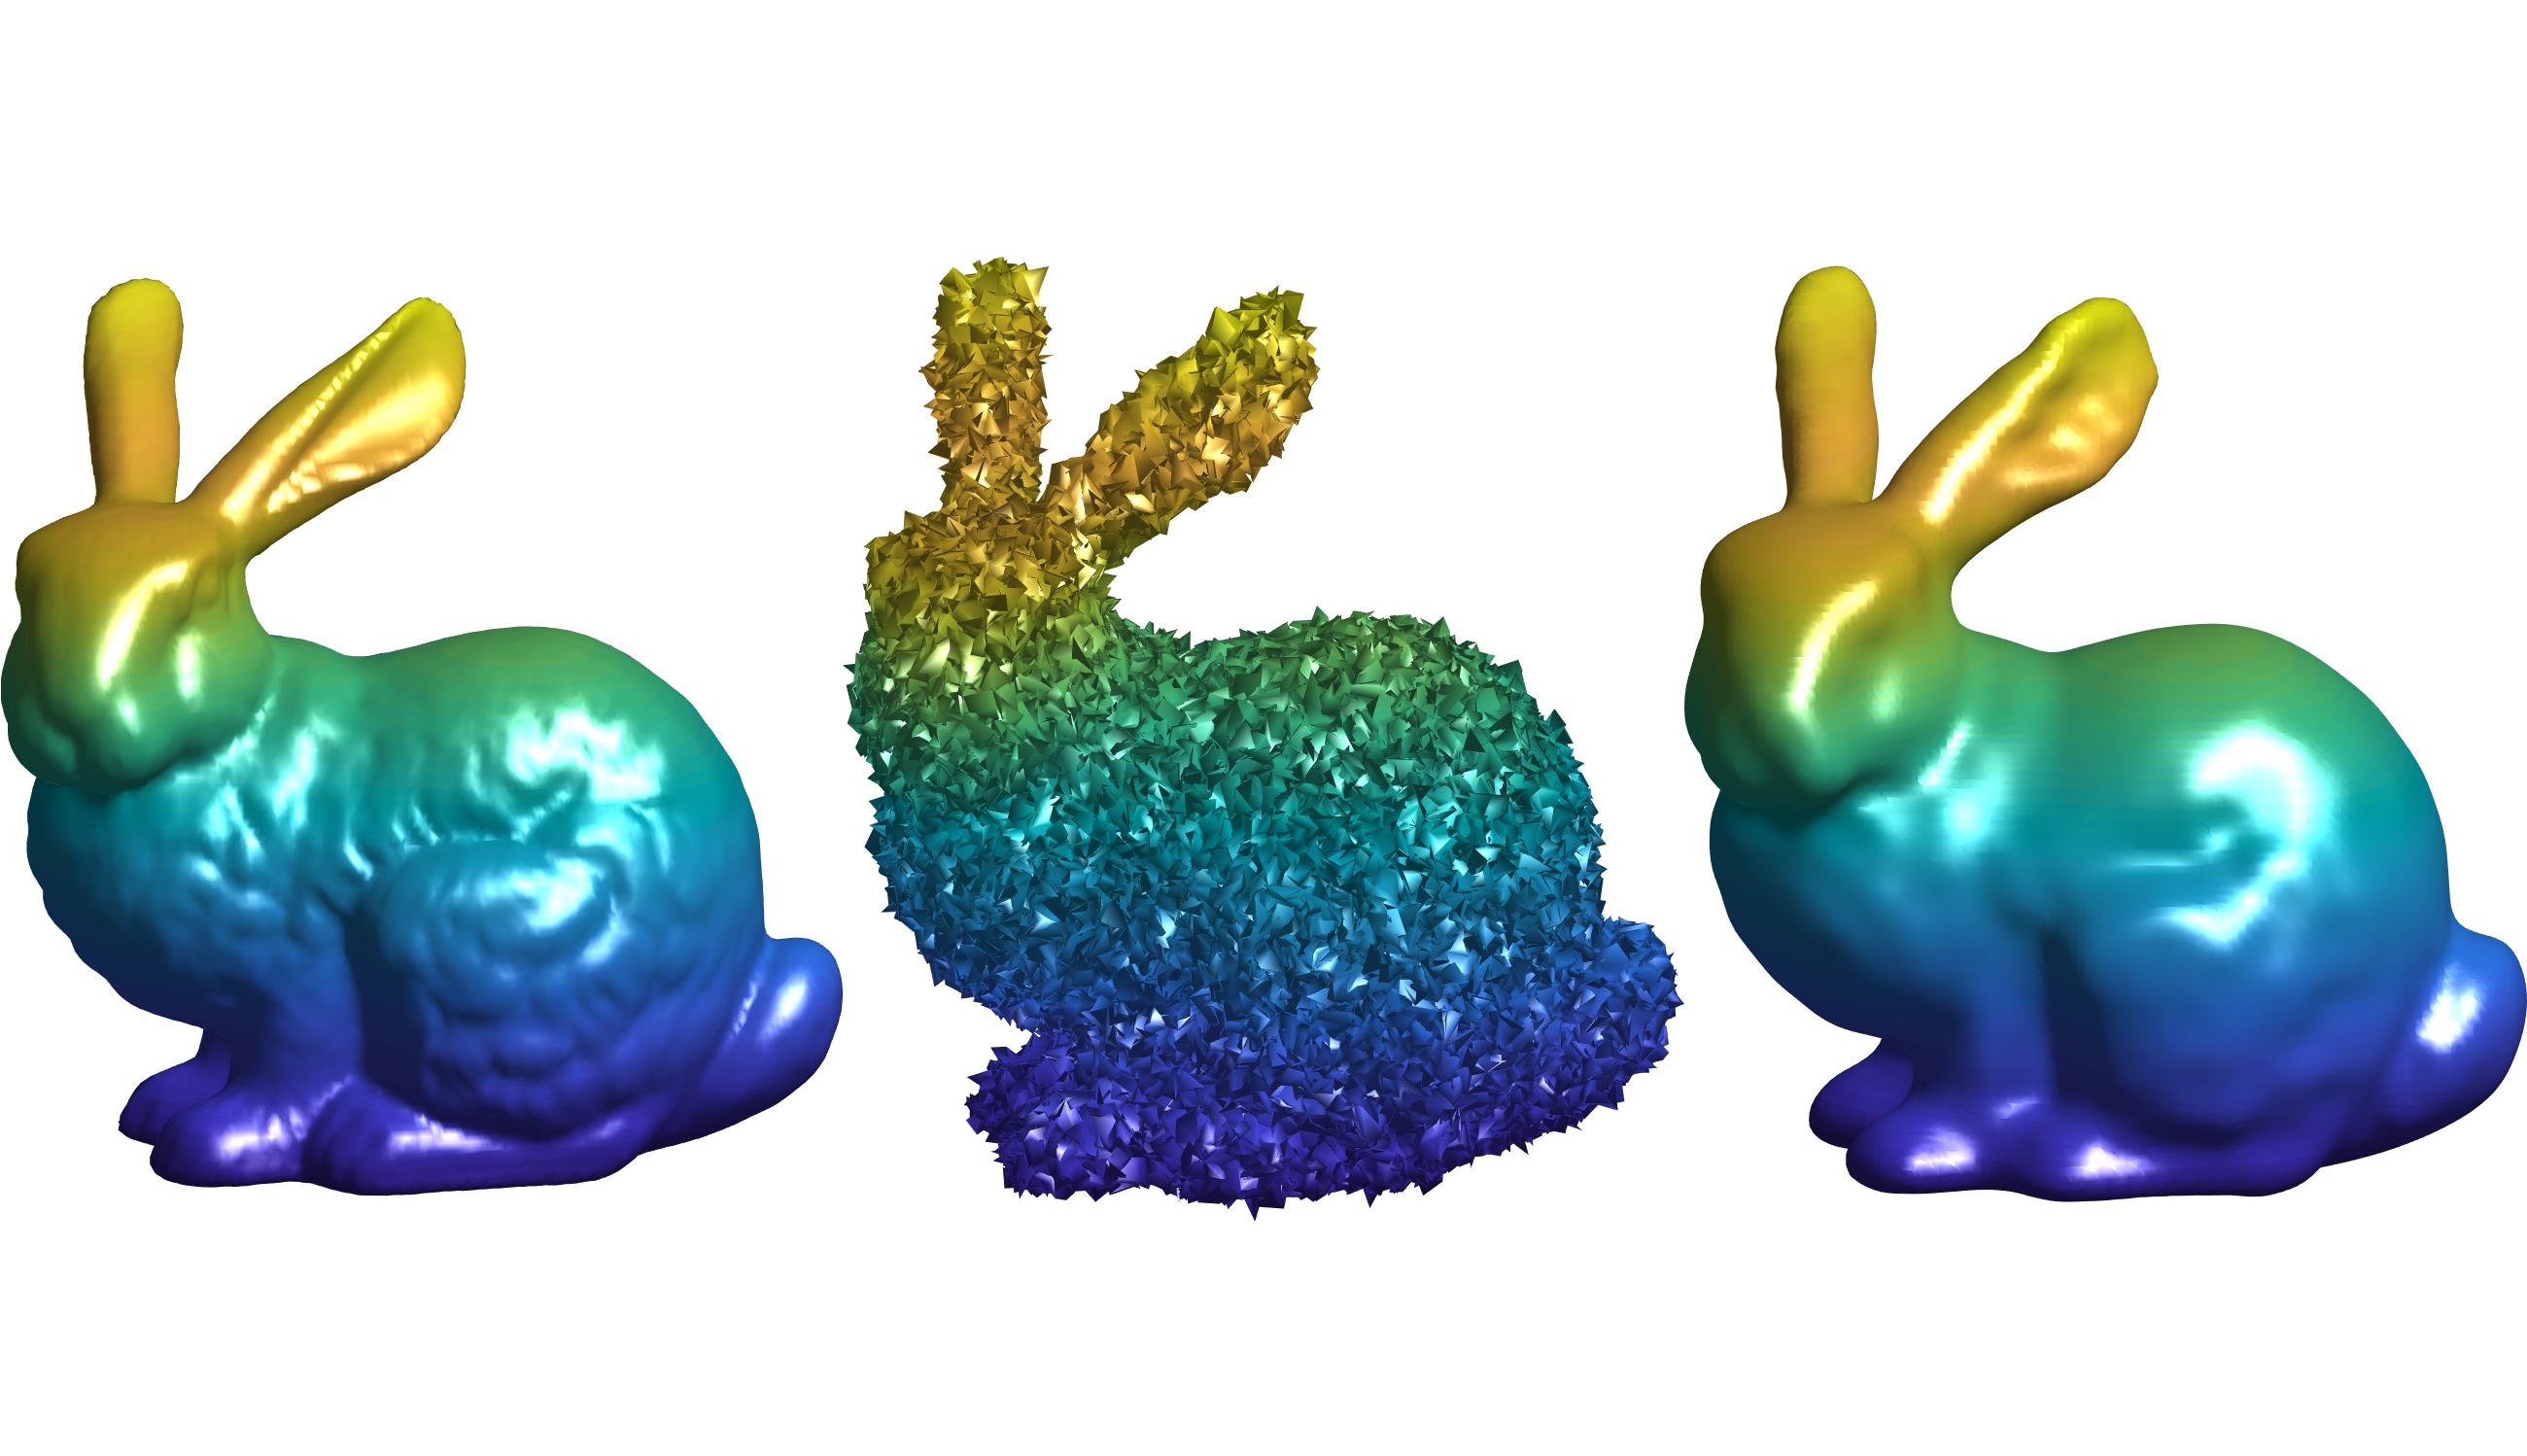
\includegraphics[width=\textwidth]{./sgpd/pics/bunny}
    \caption{(Left) Original surface (Middle) Noisy surface (Right) SKI
    reconstruction from noisy surface ($s=0.4,\,\sigma=0.12$).}\label{fig:bunny}
  \end{center}
\end{figure}

In Figure \ref{fig:bunny}, we fit the Stanford bunny using $25000$ points and
associated normals, leading to a $K^{\nabla}$ matrix of dimension $10^5$,
clearly far too large for exact training. We therefore use SKI with the
thin-plate spline kernel, with a total of 30 grid points in each dimension. The
left image is a ground truth mesh of the underlying point cloud and normals. 
The middle image shows the same mesh, but with heavily noised points and
normals. Using this noisy data, we fit a GP and reconstruct a surface shown in
the right image, which looks very close to the original.

\subsection{Bayesian optimization with derivatives}

Prior work examines Bayesian optimization (BO) with derivative information in
low-dimensional spaces to optimize model hyperparameters \citep{wu2017bayesian}.
Wang et al.~consider high-dimensional BO (without gradients) with random
projections uncovering low-dimensional structure~\citep{wang2013bayesian}. We
propose BO with derivatives and dimensionality reduction via active subspaces,
detailed in Algorithm 1.

\algorithmnormal{
  \SetKwInput{KwInput}{Input}
  \SetKwInput{KwOutput}{Output}
  \DontPrintSemicolon
  \While{Budget not exhausted}{
    Calculate active subspace projection $P \In \mathbb{R}^{D \times d}$ using
    sampled gradients\;
    Optimize acquisition function,  $u_{n+1} = \text{arg max }\mathcal{A}(u)$
    with $x_{n+1} = Pu_{n+1}$\;
    Sample point $x_{n+1}$, value $f_{n+1}$, and gradient $\nabla f_{n+1}$\;
    Update data $\mathcal{D}_{i+1} = \mathcal{D}_i \cup \{ x_{n+1}, f_{n+1},
    \nabla f_{n+1}\}$\;
    Update hyperparameters of GP with gradient defined by kernel $k(P^Tx,
    P^Tx')$\;
  }
  \caption{BO with derivatives and active subspace learning}\label{alg:BO}
}

Algorithm 1 estimates the active subspace and fits a GP with derivatives in the
reduced space.  Kernel learning, fitting, and optimization of the acquisition
function all occur in this low-dimensional subspace.  In our tests, we use the
expected improvement (EI) acquisition function, which involves both the mean and
predictive variance.  We consider two approaches to rapidly evaluate the
predictive variance $v(x) = k(x,x)-\K{xX} \Ktil{}^{-1} \K{Xx}$ at a test point
$x$.  In the first approach, which provides a biased estimate of the predictive
variance, we replace $\K{}^{-1}$ with the preconditioner solve computed by
pivoted Cholesky; using the stable QR-based evaluation algorithm, we have
\begin{equation}\label{eqn:qrpred}
  v(x) \approx \hat{v}(x) \equiv k(x,x) - \sigma^{-2} (\norm{\K
  {Xx}}^2-\norm{Q_1^T \K{Xx}}^2)\,.
\end{equation}
We note that the approximation $\hat{v}(x)$ is always a (small) overestimate of
the true predictive variance $v(x)$. In the second approach, we use a randomized
estimator as in~\cite{Bekas:2007:EDM} to compute the predictive variance at many
points $X'$ simultaneously, and use the pivoted Cholesky approximation as a
control variate to reduce the estimator variance:
\begin{equation}\label{eqn:predcv}
  v_{X'} = \diag(\K{X'X'}) - \BBE_z\left[z \odot (\K{X'X} \Ktil{}^{-1} \K{XX'}z
  - \K{X'X} M^{-1} \K{XX'} z)\right] -\hat{v}_{X'}\,.
\end{equation}
The latter approach is unbiased, but gives very noisy estimates unless many
probe vectors $z$ are used.  Both the pivoted Cholesky approximation to the
predictive variance and the randomized estimator resulted in similar optimizer
performance in our experiments.
 
\begin{figure}[ht]
  \begin{center}
    \begin{subfigure}{0.47\textwidth}
      \centering
      \captionsetup{justification=centering}
      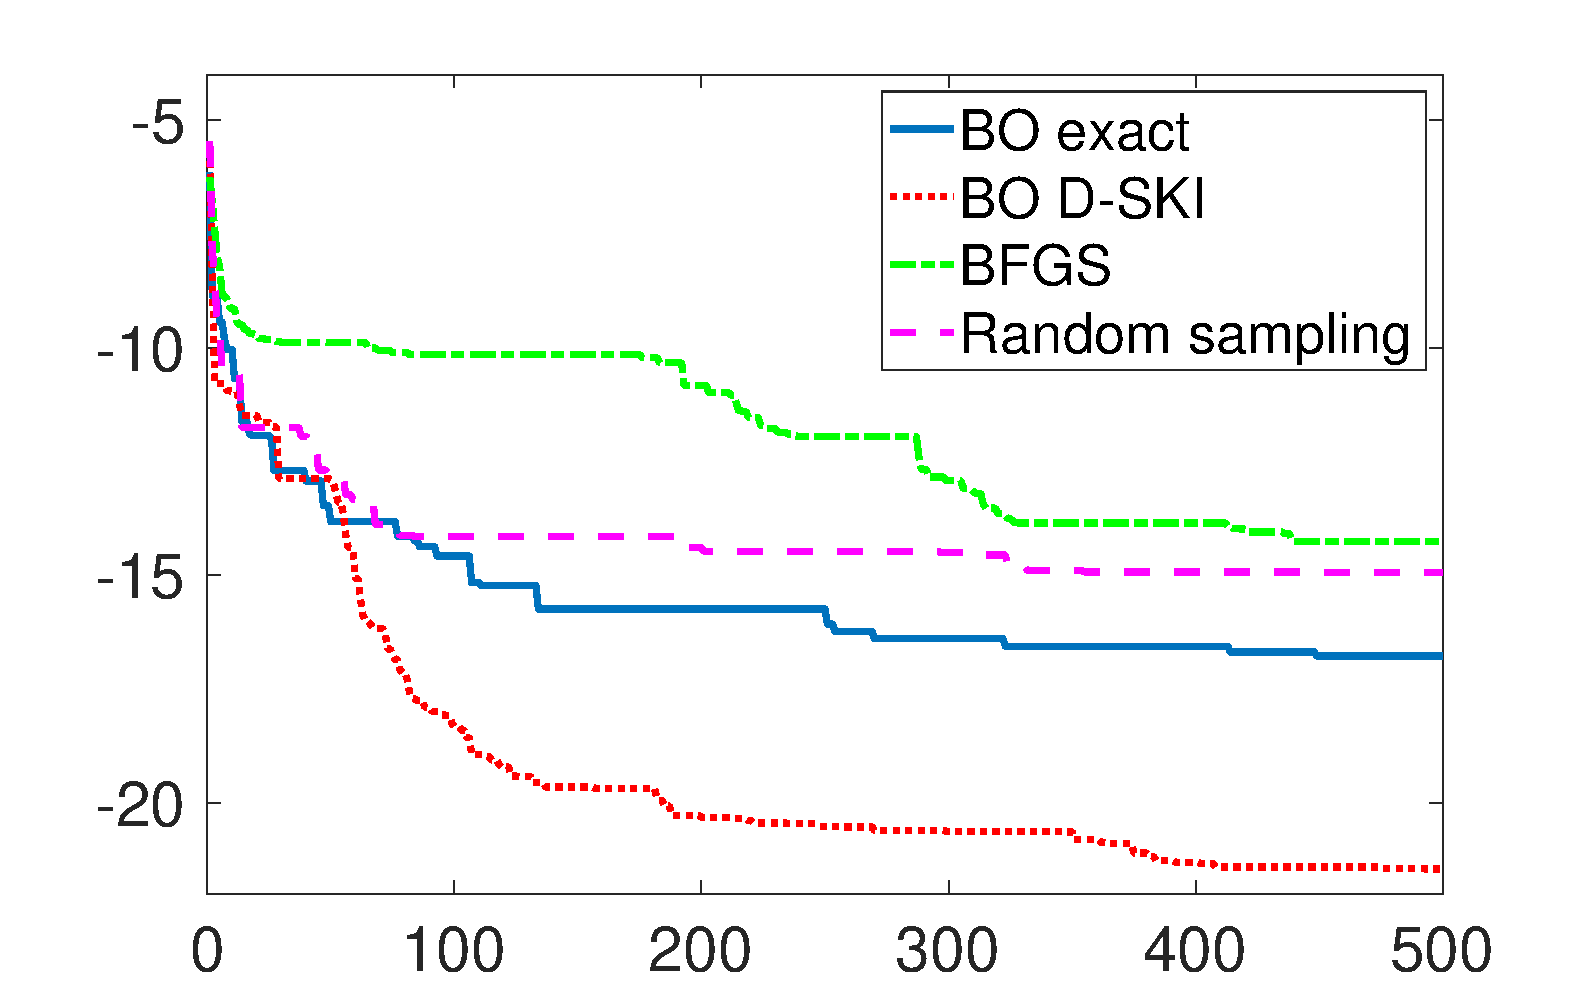
\includegraphics[width=\textwidth,trim=1.5cm 0cm 1.5cm 1cm,clip]
      {./sgpd/pics/ackley_50_5}
      \caption{BO on Ackley}\label{fig:bo_ack}
    \end{subfigure}
    \begin{subfigure}{0.47\textwidth}
      \centering
      \captionsetup{justification=centering}
      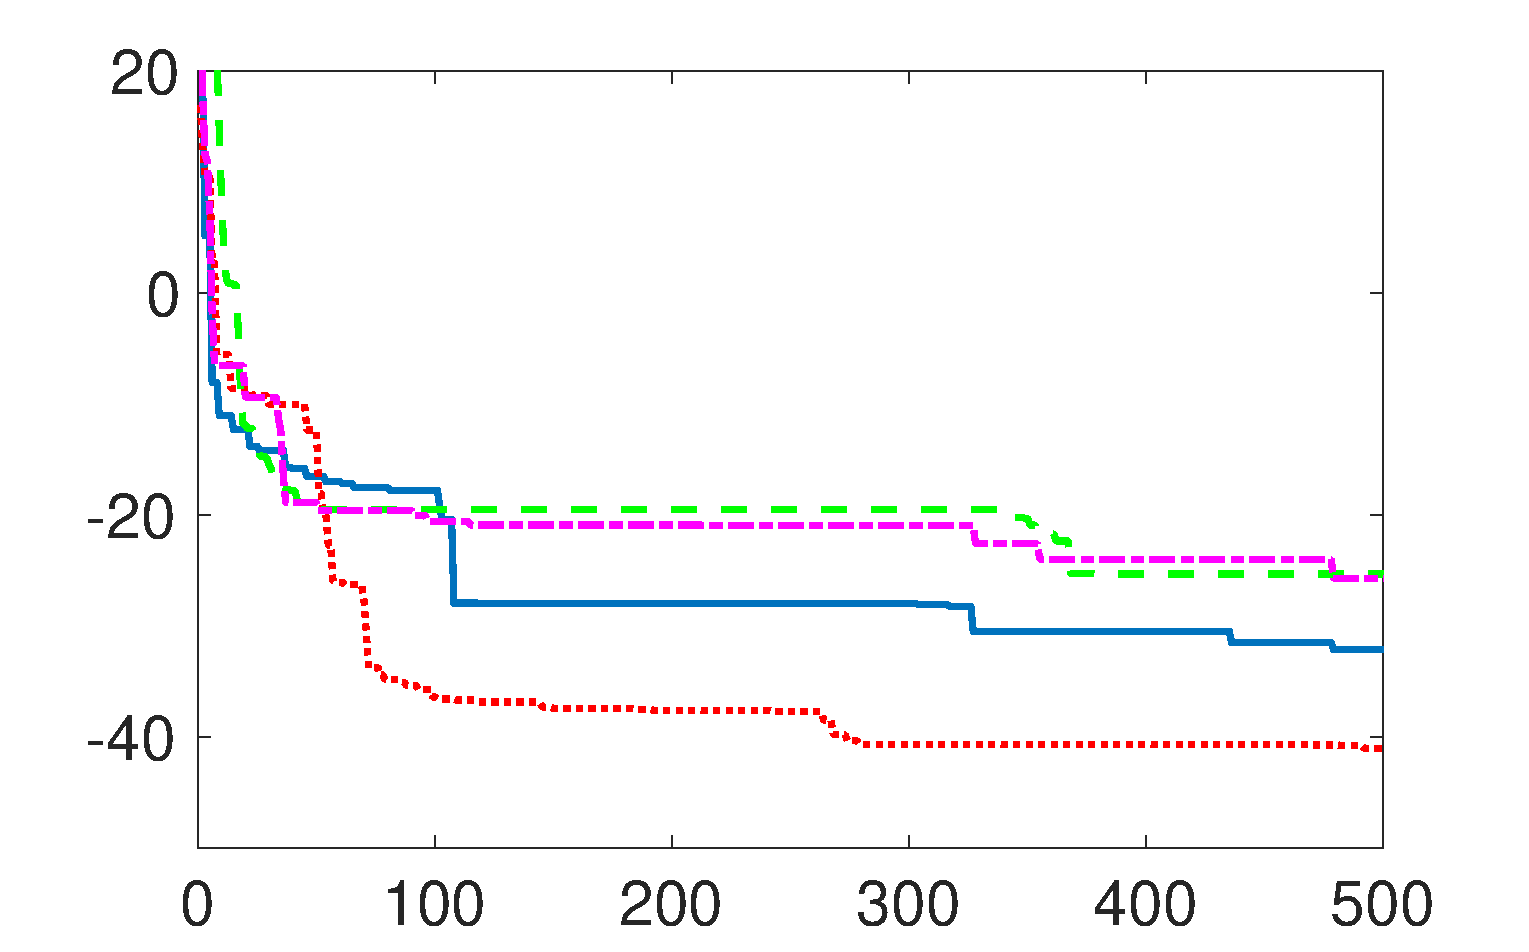
\includegraphics[width=\textwidth,trim=1.5cm 0cm 1.5cm .5cm,clip]
      {./sgpd/pics/rastrigin_50_5}
      \caption{BO on Rastrigin}\label{fig:bo_ras}
    \end{subfigure}
    \caption{In the following experiments, 5D Ackley and 5D Rastrigin are
    embedded into 50 a dimensional space. We run Algorithm 1, comparing it with
    BO exact, multi-start BFGS, and random sampling. D-SKI with active subspace
    learning clearly outperforms the other methods.}\label{fig:bo}
  \end{center}
\end{figure}

To test Algorithm 1, we mimic the experimental set up in 
\cite{wang2013bayesian}: we minimize the 5D Ackley and 5D Rastrigin test
fuctions \cite{sfutest2013}, randomly embedded respectively in $[-10, 15]^{50}$
and $[-4, 5]^{50}$. We fix $d=2$, and at each iteration pick two directions in
the estimated active subspace at random to be our active subspace projection
$P$. We use D-SKI as the kernel and EI as the acquisition function. The results
of these experiments are shown in Figure \ref{fig:bo_ack} and \cref{fig:bo_ras},
in which we compare Algorithm 1 to three other baseline methods: BO with EI and
no gradients in the original space; multi-start BFGS with full gradients; and
random search. In both experiments, the BO variants perform better than the
alternatives, and our method outperforms standard BO.